\section{VCO: Voltage Controlled Oscillator}
Esta secci\'on se propone el dise\~no de un oscilador de se\~nales senoidales cuya frecuencia pueda ser controlada por una tensi\'on de entrada,
de forma tal que para un dado rango de tensiones, se pueda producir la se\~nal deseada que var\'ie en un rango esperado de frecuencias.
En la Fig. \ref{fig:esquema_general_ejercicio_3} se ilustra un esquema general del sistema deseado.

\begin{figure}[H]
    \centering
    \includegraphics[scale=0.5]{../EJ3/Recursos/system_scheme.png}
    \caption{Esquema general del sistema propuesto}
    \label{fig:esquema_general_ejercicio_3}
\end{figure}


\subsection{Introducci\'on te\'orica}
El objetivo de esta introducci\'on es establecer las bases te\'oricas sobre las cuales se construye
el an\'alisis desarrollado para el dise\~no del sistema propuesto. No obstante, se asume que el lector posee
una base te\'orica sobre algunos conceptos, lo cual se ir\'a indicando a lo largo de tal an\'alisis.

\subsubsection{Distorsi\'on Arm\'onica}
La teor\'ia de series generalizadas de Fourier establece que cualquier se\~nal peri\'odica, es decir una funci\'on dada tal que
$f: I\!R -> I\!R$ que cumple tener un per\'iodo fundamental dado $f(t + T) = f(t)$, con T perteneciente a los reales positivos, puede
ser proyectada sobre un espacio vectorial descripto por su base ortonormal.
En otras palabras, la serie trigonométrica de Fourier como caso particular permite describir un se\~nal peri\'odica como combinaci\'on 
lineal de funciones seno y coseno. Se suele denominar a cada una de estas componentes como arm\'onicos cuyas frecuencias son m\'ultiplos de la 
frecuencia fundamental, y desde un punto de vista espectral es sencillo observar la distribuci\'on de potencia de la se\~nal para cada frecuencia
arm\'onica.

\begin{figure}[H]
    \centering
    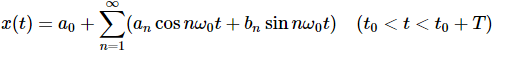
\includegraphics[scale=0.6]{../EJ3/Recursos/fourier_series.PNG}
    \caption{Series de Fourier}
\end{figure}


\begin{figure}[H]
    \centering
    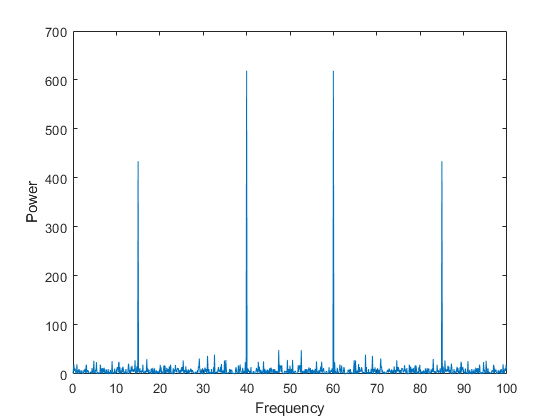
\includegraphics[scale=0.4]{../EJ3/Recursos/BasicSpectralAnalysisExample_01.png} 
    \caption{Espectro en frecuencia}
\end{figure}

La distorsi\'on arm\'onica puede ser entendida como la presencia de arm\'onicos no deseados que en el dominio temporal alteran o distorsionan la forma
de onda esperada, esto puede pasar como consecuencia del uso de sistemas no lineales o por el l\'imite f\'isico de ancho de banda que suelen tener
los circuitos, aunque no siempre se vuelve apreciable su efecto sobre la eliminaci\'on de los arm\'onicos deseados.
As\'i, una se\~nal senoidal pura \'unicamente contiene su arm\'onico fundamental, y en t\'erminos del espectro en frecuencia s\'olo una componente. Esto permite
estudiar la distorsi\'on de tales se\~nales analizando aquellos componentes arm\'onicos no deseados que pueden aparecen, y se utiliza la expresi\'on de la Ec. \ref{eq:distorsion_de_armonico}
para cuantificarla. La distorsi\'on total se define como se observa en la Ec. \ref{eq:total_distorsion}.

\begin{equation}
    HD_n = \frac{armonico_n}{armonico_{fundamental}}
    \label{eq:distorsion_de_armonico}
\end{equation}

\begin{equation}
    THD = \sqrt{\sum_{n} (HD_n)^{2}}
    \label{eq:total_distorsion}
\end{equation}

\subsubsection{Jitter}
Se define el Jitter como la desviaci\'on pr\'actica del per\'iodo de una se\~nal respecto de su valor te\'orico esperado. Este es un aspecto
a tener en cuenta en el dise\~no y an\'alisis de osciladores, y puede clasificarse generalmente seg\'un si es aleatorio o determin\'istico.

\begin{figure}[H]
    \centering
    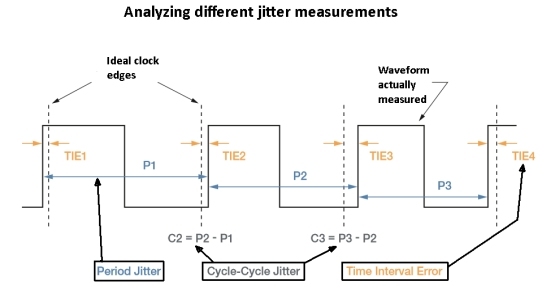
\includegraphics[scale=0.5]{../EJ3/Recursos/different-jitter-measurements.jpg}
    \caption{Diagrama del Jitter medido en un per\'iodo o entre ciclos}
    \label{fig:jitter_diagram}
\end{figure}

El jitter aleatorio corresponde a la desviaci\'on del per\'iodo provocada por el ruido t\'ermico que generan los componentes resistivos en la pr\'actica.
Por otro lado, el jitter determin\'istico consiste en analizar las posibles desviaciones temporales, ya sea de un per\'iodo respecto del valor real, as\'i
como entre per\'iodos de ciclos consecutivos. Esto puede observarse en la Fig. \ref{fig:jitter_diagram}.

\subsection{An\'alisis de circuitos}
Se busca realizar un an\'alisis de los circuitos empleados posteriormente en el dise\~no para facilitar, no s\'olo este proceso,
sino la divisi\'on en etapas seg\'un lo requiera el sistema, teniendo en cuenta las fortalezas y debilidades de cada una de ellas.

\subsubsection{Acondicionamiento lineal de se\~nal}
En la pr\'actica suele ser necesario realizar un acondicionamiento lineal de una se\~nal de entrada, esto implica matem\'aticamente aplicar un desplazamiento
y un escalaje sobre la magnitud de entrada, adaptando el rango de valores de entrada a un rango aceptable de salida. Se propone como circuito para realizar esta transformaci\'on
de las magnitudes, el ilustrado en la Fig. \ref{fig:circuito_acondicionamiento_lineal}.

\begin{figure}[H]
    \centering
    \includegraphics[scale=0.55]{../EJ3/Recursos/circuito_acondicionamiento_lineal.png}
    \caption{Acondicionamiento lineal de se\~nales}
    \label{fig:circuito_acondicionamiento_lineal}
\end{figure}

Se plantean las siguientes ecuaciones, donde se define la salida del amplificador operacional configurado como buffer o seguidor de tensi\'on $V_{OFF}$.

\begin{align*}
    & V_{OFF} = \frac{V_{CC} \cdot R_2}{R_1 + R_2} \\
    & V_o = V_i \cdot \frac{R_4}{R_3 + R_4} \cdot \frac{R_5 + R_6}{R_5}
    + V_{OFF} \cdot \frac{R_3}{R_3 + R_4} \cdot \frac{R_5 + R_6}{R_5}
\end{align*}

Aplicando como criterio para simplificar el manejo algebraico, resulta pr\'actico establecer que se cumpla la condici\'on
$R_3 = R_5$ y $R_4 = R_6$.

\begin{equation}
    V_o = V_i \cdot \frac{R_4}{R_5} + V_{OFF}
\end{equation}

En conclusi\'on, este circuito con esta \'ultima expresi\'on permite de manera sencilla realizar una transformaci\'on que permita adaptar o acondicionar
la se\~nal entrante, conociendo la pendiente y ordenada al origen que se desean como salida. Es importante mencionar que el circuito no garantiza un l\'imite de tensi\'on 
que no sea el de saturaci\'on de los amplificadores, con lo cual a menos que se haga uso de este, ser\'a necesario un circuito limitador de tensi\'on en la salida seg\'un el caso.

\subsubsection{Comparador Schmitt Trigger inversor}
El comparador Schmitt Trigger es una configuraci\'on del amplificador operacional utilizando una realimentaci\'on regenerativa o positiva,
que lo que busca es crear un comparador con hist\'eresis para prevenir fluctuaciones u oscilaciones en la salida del mismo por el efecto de se\~nales
con contenido no deseado de ruido. Estas configuraciones vienen en la forma de inversoras o no inversoras, y establecen dos l\'imites de comparaci\'on
para determinar estado alto o estado bajo, y cuando no se emplea un corrimiento por offset, se encuentran sim\'etricas al cero.

\begin{figure}[H]
    \centering
    \includegraphics[scale=0.7]{../EJ3/Recursos/diagrama_schmitt_trigger.png}
    \caption{Diagrama del comparador con hist\'eresis}
    \label{fig:diagrama_schmitt_trigger}
\end{figure}

En la Fig. \ref{fig:diagrama_schmitt_trigger} se puede observar la funci\'on de $V_o = f(V_i)$ del comparador Schmitt Trigger inversor,
para el cual se propone el circuito de la Fig. \ref{fig:circuito_schmitt_trigger}.

\begin{figure}[H]
    \centering
    \includegraphics[scale=0.6]{../EJ3/Recursos/schmitt_trigger.png}
    \caption{Circuito Schmitt Trigger inversor}
    \label{fig:circuito_schmitt_trigger}
\end{figure}

Se plantea el potencial en las dos entradas del amplificador operacional, y dado que la transici\'on se da en torno al encuentro
de ambos valores de tensi\'on, se igualan las expresiones y asumiendo estados alto y bajo de salida, se encuentra la expresi\'on
de los valores de comparaci\'on.

\begin{align*}
    & V^{+} = V_o \cdot \frac{R_1}{R_1 + R_2} \\
    & V^{-} = V_i \\
    & \Rightarrow V_T = V_{CC_{SAT}} \cdot \frac{R_1}{R_1 + R_2}
\end{align*}

\subsubsection{Voltage Controlled Oscillator}
En la Fig. \ref{fig:circuito_vco} se puede observar el circuito propuesto para realizar el armado de un VCO utilizando dos amplificadores operacionales
y un MOSFET. Se realiza un an\'alisis considerando un comportamiento ideal de los amplificadores, y asumiendo que el lector tiene un conocimiento del 
funcionamiento del transistor.

\begin{figure}[H]
    \centering
        \includegraphics[scale=0.5]{../EJ3/Recursos/circuit_vco.png}
    \caption{Circuito de un Voltage Controlled Oscillator}
    \label{fig:circuito_vco}
\end{figure}

\paragraph{Operaci\'on del circuito:} Se utiliza una configuraci\'on de amplificador operacional para poder integrar una se\~nal cuadrada,
de esta forma se produce una se\~nal triangular, no obstante, para poder garantizar que la frecuencia sea controlada por la tensi\'on de entrada,
el valor de corriente que determina los tiempos de carga y descarga depende de la tensi\'on de entrada. De esta forma, a corriente constante la carga del capacitor
se da linealmente hasta encontrarse con los extremos de comparaci\'on de la configuraci\'on schmitt trigger inversora, que produce en funci\'on de ello una onda
cuadrada sincronizada que conmuta un transistor para lograr cambiar el sentido de corriente, y por ende, de carga del capacitor.

\paragraph{Comparador Schmitt Trigger inversor:} De la comprensi\'on cualitativa del funcionamiento del VCO, se puede ver que el comparador
produce una onda cuadrada a partir de la triangular, pero adem\'as su funcionalidad principal est\'a en determinar el valor pico de tensi\'on de la onda triangular.
Sea $V_x$ la tensi\'on pico de la triangular, luego se puede determinar este valor utilizando el an\'alisis ya hecho del schmitt trigger, entonces:

\begin{equation}
    V_x = V_{CC_{SAT}} \cdot \frac{R_6}{R_6 + R_7}
    \label{eq:ecuacion_tensiones_vco}
\end{equation}

\paragraph{Integrador controlado por tensi\'on:} Si inicialmente se ignora la presencia del MOSFET y se lo considera una llave ideal, asumiendo que $R_2 = R_3$,
luego se puede determinar que la corriente $I_{R_1} = \frac{V_i}{2 \cdot R_1}$ se mantiene siempre constante, y cuando la llave est\'e conectada circular\'a por $R_4$ una corriente $I_{R_4} = \frac{V_i}{2 \cdot R_4}$. Dado que el capacitor se carga con una corriente $I_C = I_{R_1} - I_{R_4}$, luego
se deduce que $R_4 = \frac{R_1}{2}$, dado que de esta forma se cumplir\'a que la llave al estar conectada o no, s\'olo cambia el sentido de la corriente del capacitor,
pero su magnitud se mantiene constante. De esta forma se integra y calcula la tensi\'on de salida como:

\begin{equation*}
    i_c(t) = C \cdot \frac{\delta V_c(t)}{\delta t} \Rightarrow \int_0^{t} V_c(t) = \int_0^{t} \frac{i_C(t) \cdot \delta_t}{C}
\end{equation*}

\begin{equation}
    V_c(t) = V_c(0) + \frac{i_C}{C} \cdot t \Rightarrow V_c(t) = V_c(0) + \frac{V_i}{2 \cdot R_1 \cdot C} \cdot t
\end{equation}

\paragraph{Expresi\'on del VCO:} Finalmente, considerando que tal pendiente est\'a dada por el cociente entre la tensi\'on pico a pico
de la triangular y la mitad de su per\'iodo, se puede despejar una expresi\'on que vincula linealmente la tensi\'on de entrada con la frecuencia de la se\~nal de salida. Esto es, la ecuaci\'on que caracterizar\'a el funcionamiento
del VCO.

\begin{equation*}
    \frac{V_{PP} \cdot 2}{T} = \frac{V_i}{2 \cdot C \cdot R_1}
\end{equation*}

\begin{equation}
    f = V_i \cdot \frac{1}{8 \cdot V_x \cdot R_1 \cdot C}
    \label{eq:ecuacion_caracteristica_vco}
\end{equation}

\paragraph{Comentarios pr\'acticos:} Para el circuito propuesto se desea utilizar un transistor de tecnolog\'ia MOSFET dado que de esta forma se garantiza que operando en regi\'on lineal,
la resistencia del canal formado ser\'a peque\~na en comparaci\'on con $R_4$, logrando as\'i que el error por asimetr\'ia de la onda introducido como consecuencia de una asimetr\'ia entre las corrientes
de carga y descarga, sea peque\~no.

\paragraph{Observaciones:} Durante el an\'alisis te\'orico del circuito, se observ\'o que las limitadas funcionalidades que se le dan al generador a dise\~nar podr\'ian se expandidas. En otras palabras,
podr\'ia emplearse una llave selectora de capacitores m\'ultiplos por 10 entre s\'i, logrando as\'i cambiar el rango de frecuencias a generar. Por otro lado, se podr\'ian colocar etapas de salida de las ondas
generadas para poder modificar la amplitud y el nivel de continua u offset. Finalmente, para modificar el duty de la onda cuadrada o la simetr\'ia de la onda triangular bastar\'ia
con utilizar un preset o potenciometro para modificar las corrientes en las mallas de entrada.

\subsubsection{Conversor triangular a senoidal}

\paragraph{Concepto general:} En t\'erminos te\'oricos, el proceso de conversi\'on de una se\~nal triangular a senoidal es una transformaci\'on que puede ser procesada por un sistema
cuya funci\'on transferencia no lineal debe ser como se describe en la Ec. \ref{eq:modelo_matematico_conversor}. En otras palabras, se debe modelizar esta funci\'on la cual realiza
un mapeo de la se\~nal lineal de entrada sobre el senoide de salida. Es importante destacar, que la frecuencia siempre estar\'a dada por la se\~nal de entrada y la amplitud por el sistema.

\begin{equation}
    X_o = K_1 \cdot \sin{(K_2 \cdot X_i)}
    \label{eq:modelo_matematico_conversor}
\end{equation}

\paragraph{Modelo circuital te\'orico:} En Junio de 1976, Robert G. Meyer, Willy Sanken, y otros colaboradores publicaron un paper en IEEE sobre una investigaci\'on que llevaron a cabo por sugerencia de un colega, sobre la posibilidad de implementar esta funci\'on
descripta anteriormente, empleando un amplificador diferencial con transistores bipolares de juntura. En la Fig. \ref{fig:conversor_teorico_meyer} se puede observar el esquema te\'orico propuesto.

\begin{figure}[H]
    \centering
    \includegraphics[scale=0.5]{../EJ3/Recursos/conversor_teorico_meyer.png}
    \caption{Circuito te\'orico del conversor de Meyer}
    \label{fig:conversor_teorico_meyer}
\end{figure}

En forma sintetizada, se puede demostrar que la corriente que circula por la resistencia $R$ sigue un comportamiento en funci\'on de la tensi\'on de entrada que se ve descripto
por una ecuaci\'on con una funci\'on logar\'itmica. Si se calculan las series de Taylor de dicha funci\'on logar\'itmica, de la funci\'on senoidal de la Ec. \ref{eq:modelo_matematico_conversor},
luego se puede encontrar que ambas funciones puede, bajo ciertas condiciones, compartir los primeros cinco t\'erminos de tales series, con lo cual se obtendr\'ia una buena aproximaci\'on senoidal. 
Para lograr esto \'ultimo, Meyer dedujo que era necesario que se cumpliera:

\begin{align}
    & I \cdot R \approx 2.5 \cdot V_T \\
    & V_{i_{P}} = V_T \cdot 6.6 \\
    & V_T = \frac{k_B \cdot T}{q}
\end{align}


En conclusi\'on, si se logra que la entrada del circuito sea una se\~nal triangular de simetr\'ia $50\%$ con una tensi\'on pico de $172mV$, donde $I \cdot R \approx 62.5mV$. Entonces,
siguiendo estrictamente esas condiciones en los t\'erminos ideales del modelo circuital propuesto, se puede conseguir una salida senoidal con una distorsi\'on arm\'onica por debajo de $1\%$.

\paragraph{Modelo circuital pr\'actico:} Para que el circuito y las conclusiones anteriores sean aplicables en la realidad, es necesario realizar algunas modificaciones. Estas modificaciones
fueron realizadas bajo ciertos criterios, seg\'un se enumeran a continuaci\'on:

\begin{itemize}
    \item \textbf{Atenuador:} Las se\~nales triangulares conectadas, si bien deben ser de simetr\'ia $50\%$, su amplitud podr\'a variar con lo cual es necesario una etapa de ajuste para 
    llevar el valor de entrada a los $172mV$ necesario para minimizar la distorsi\'on.
    \item \textbf{Fuente de corriente compensada:} Se desea utilizar una fuente de corriente simple que entregue la corriente de ambos transistores del par diferencial, en donde se utiliza una compensaci\'on
    por variaciones de $V_{BE}$ frente a cambios bruscos de temperatura, como mecanismo de protecci\'on para mantener las caracter\'isticas del circuito.
    \item \textbf{Par diferencial:} Como se describi\'o anteriormente, es necesario un par diferencial con el cual, bajo ciertas condiciones, aproximar la respuesta de una se\~nal senoidal utilizando como resistencia $R$
    del modelo te\'orico de Meyer, un preset que se encuentra para compensar los par\'ametros constructivos de los transistores.
    \item \textbf{Fuente de corriente espejo proporcional:} Se la emplea como carga activa porque as\'i se logra mejorar la relaci\'on sim\'etrica entre corrientes de $Q_1$ y $Q_2$ y crear idealmente un punto de tierra virtual en el colector de $Q_2$,
    lo que permite tener una salida en modo com\'un. Y dado que en el modelo incremental la resistencia de tal fuente es muy grande, las corrientes incrementales se van mayoritariamente por la salida, caracterizando al amplificador
    por tener una salida de corriente, esto ser\'a aprovechado colocando a la salida una etapa de transimpedancia. Se busca que $R_4 = R_5$, emulando una fuente espejo simple, no obstante la desviaci\'on por diferencia en curvas caracter\'isticas de las junturas
    es menor con respecto al par espejo simple.
    \item \textbf{Etapa amplificador de transimpedancia:} Se utiliza un amplificador de transimpedancia aprovechando que la salida del diferencial con carga activa es de corriente, y dado que la salida est\'a montada sobre una tierra virtual,
    luego no es necesario realizar ning\'un ajuste sobre el nivel de continua u offset. La ganancia del amplificador estar\'a dada por $-R_{10} - R_{11}$ seg\'un el total de la realimentaci\'on.
\end{itemize}

\begin{figure}[H]
    \centering
    \includegraphics[scale=0.4]{../EJ3/Recursos/conversor_propuesto.png}
    \caption{Conversor triangular a senoidal propuesto}
    \label{fig:circuito_conversor_propuesto}
\end{figure}

\subsection{Dise\~no de VCO}

\subsubsection{Especificaciones y etapas}

\subsubsection{C\'alculo de componentes}

\subsubsection{Simulaci\'on y verificaci\'on}

\subsection{Resultados}

\subsubsection{Mediciones}

\subsubsection{An\'alisis de resultados}

\subsection{Conclusiones}